
This benchmark deals with the 2-D thermal convection of a fluid 
of infinite Prandtl number in a rectangular closed cell.
In what follows, I carry out the case 1a, 1b, and 1c experiments as shown in \cite{blbc89}:
steady convection with constant viscosity in a square box.

The temperature is fixed to zero on top and to $\Delta T$ at the bottom, 
with reflecting symmetry at the sidewalls (i.e. $\partial_x T=0$) 
and there are no internal heat sources. 
Free-slip conditions are implemented on all boundaries. 

The Rayleigh number is given by
\begin{equation}
Ra = \frac{\alpha g_y \Delta T h^3 }{\kappa \nu}
=\frac{\alpha g_y \Delta T h^3 \rho^2 c_p}{k \mu}
\end{equation}

In what follows, I use the following parameter values:  %, as given in \cite{krhb12}:
$L_x=L_y=1$,$\rho_0=c_P=k=\mu=1$, $T_0=0$, $\alpha=10^{-2}$, $g=10^{2}Ra$
and I run the model with $Ra=10^4,10^{5}$ and $10^6$.

The initial temperature field is given by 
\begin{equation}
T(x,y)=(1-y) - 0.01\cos(\pi x) \sin(\pi z)
\end{equation}
The perturbation in the initial temperature fields leads to 
a perturbation of the density field and sets the fluid in motion. 

Depending on the initial Rayleigh number, the system ultimately reaches a 
steady state after some time. The steady-state 
temperature fields of case 1a,b,c are shown hereunder: 

\fbox{
\parbox{10cm}{{\bf features}
\begin{itemize}
\item $Q_1\times P_0$ element
\item incompressible flow
\item penalty formulation
\item Dirichlet boundary conditions (free-slip)
\item Boussinesq approximation
\item direct solver
\item non-isothermal
\item buoyancy-driven flow
\item isoviscous
\item CFL-condition
\end{itemize}
}}

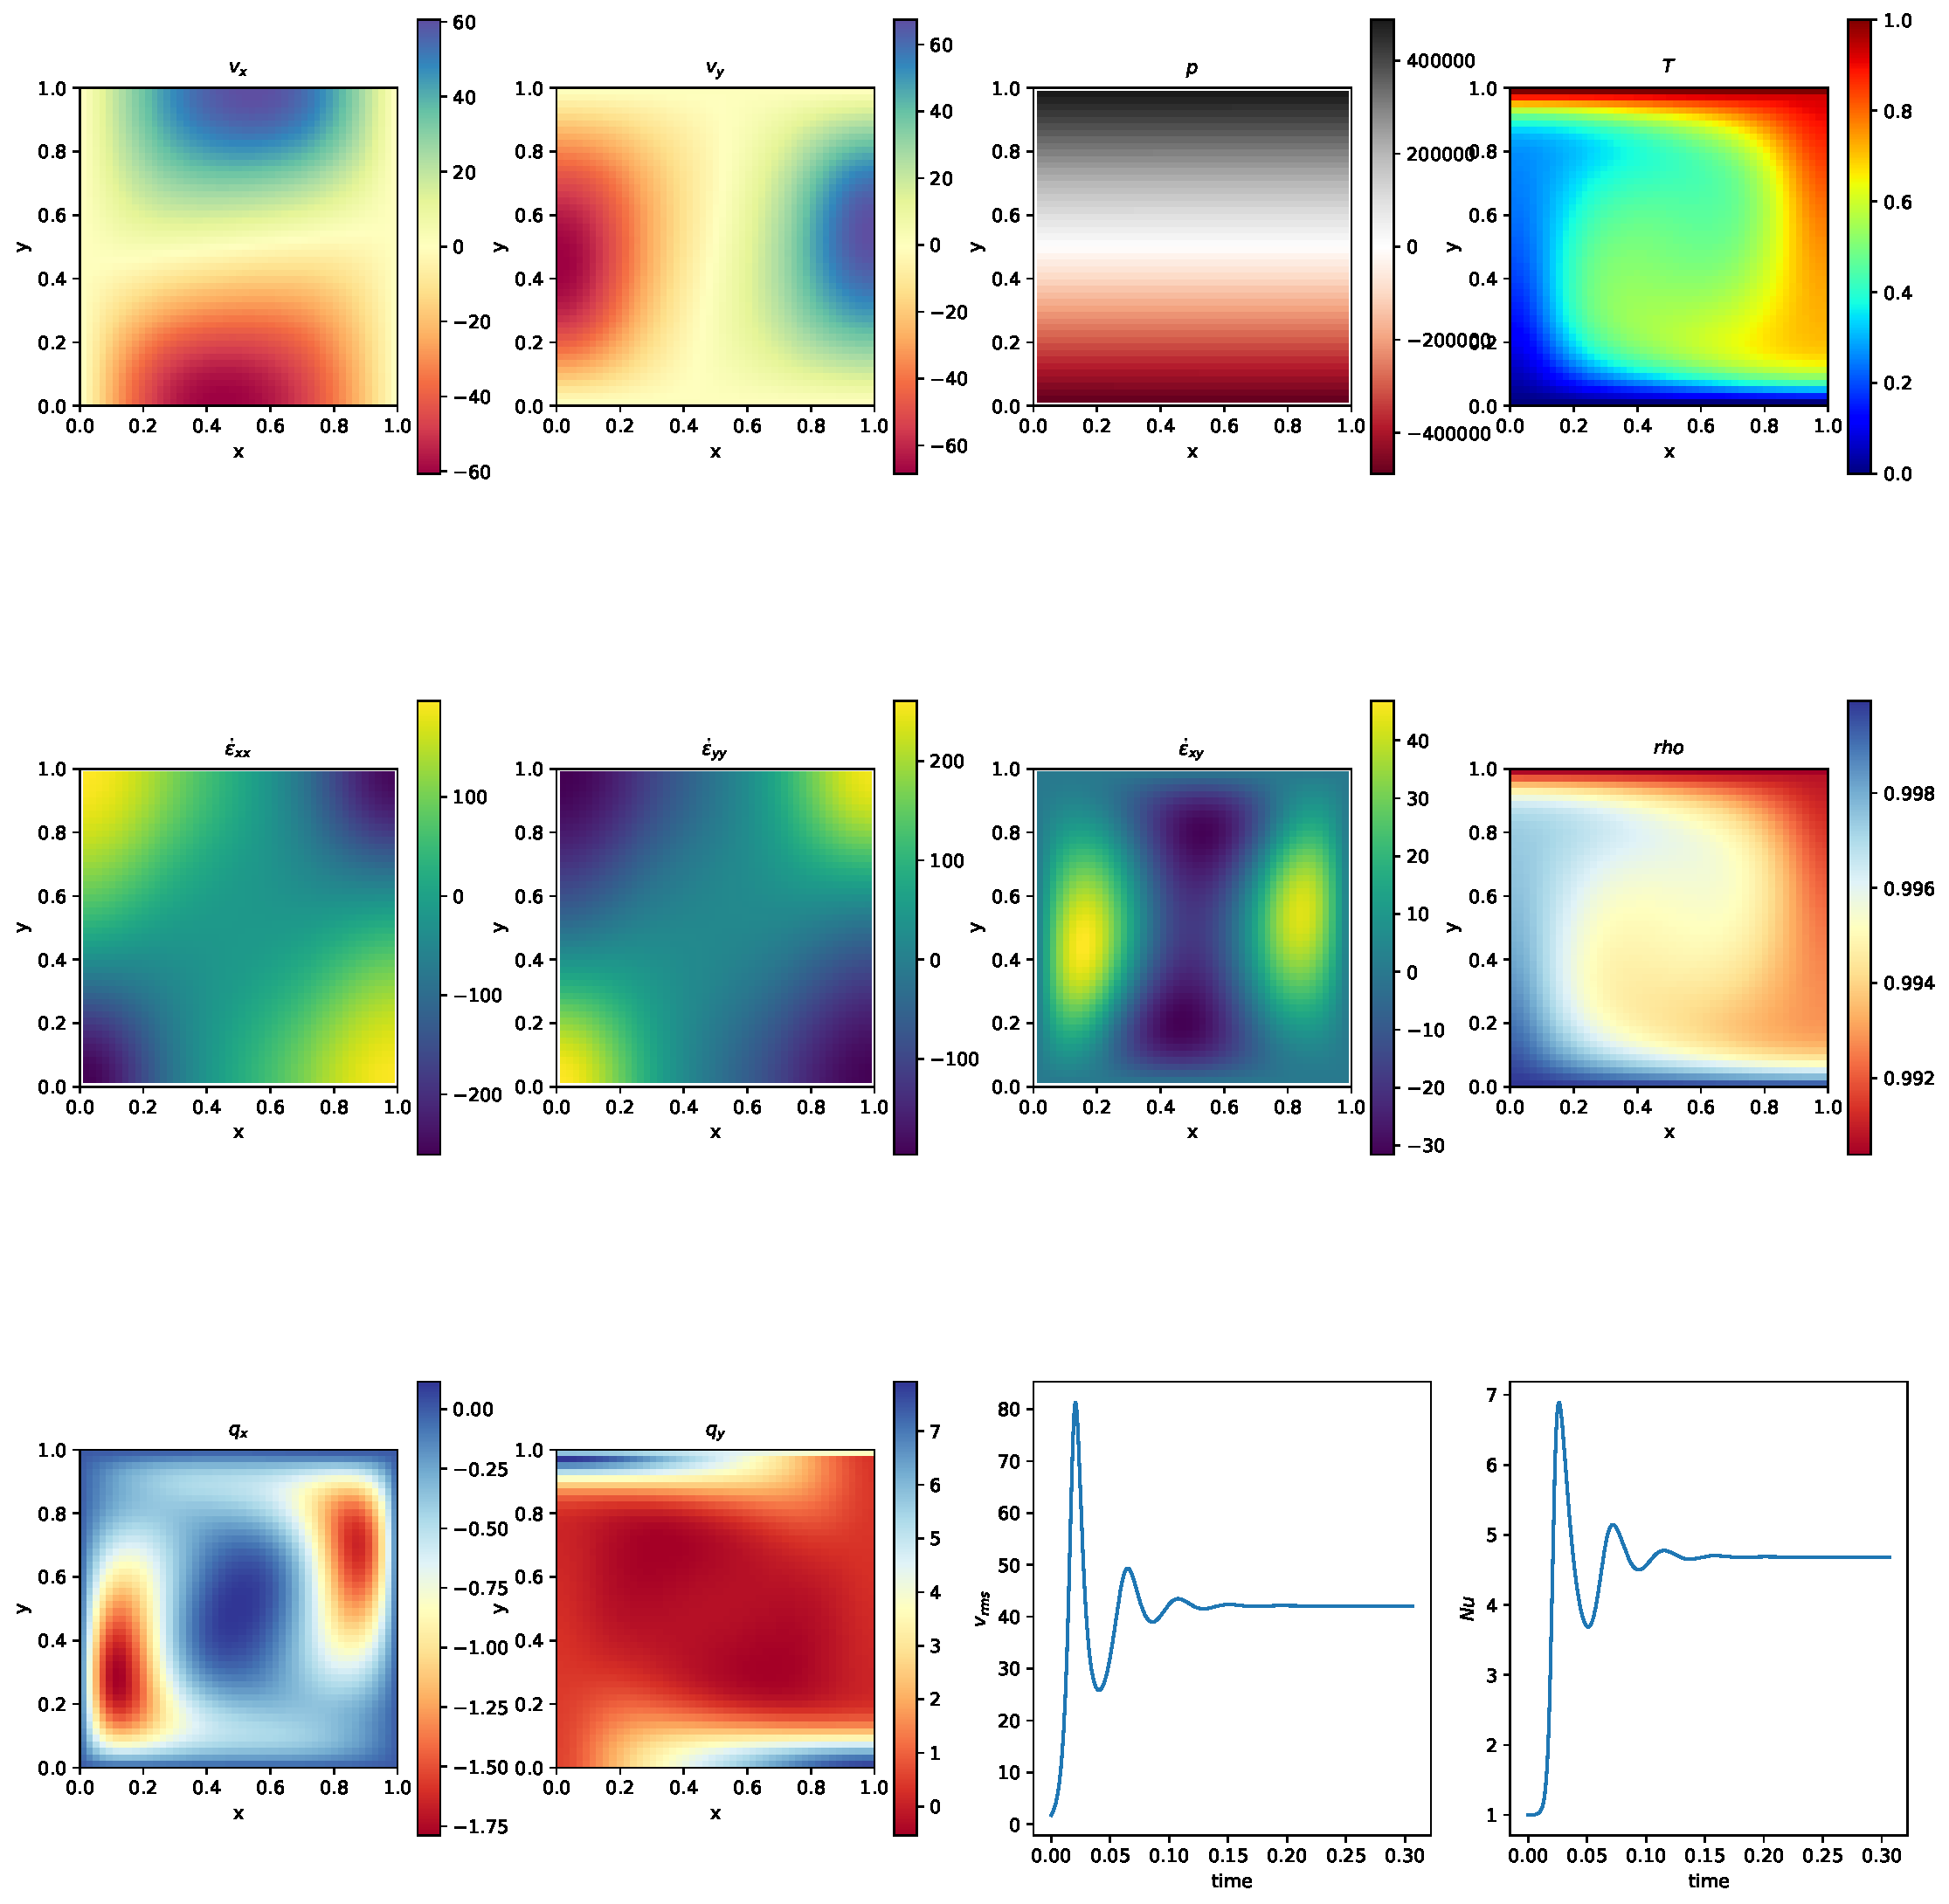
\includegraphics[width=16cm]{python_codes/fieldstone_convection_box/solution_convection_box.pdf}

ToDo:

implement steady state criterion

reach steady state

do Ra=1e4, 1e5, 1e6

plot against blankenbach paper and aspect

look at critical Ra number
